\documentclass[12pt,conference]{IEEEtran}
\usepackage{url}
\usepackage{graphicx}
\usepackage[norule]{footmisc}
\graphicspath{ {./images/} }
\usepackage{float}
\floatstyle{boxed} 
\restylefloat{figure}
\usepackage{physics}

% footer style
\makeatletter
\def\footnoterule{\kern-3\p@
  \hrule \@width 2in \kern 2.6\p@} % the \hrule is .4pt high
\makeatother

% paragraph indentation
\setlength{\parindent}{2.5em}
\setlength{\parskip}{1em}

% disable word break
\tolerance=1
\emergencystretch=\maxdimen
\hyphenpenalty=10000
\hbadness=10000




\begin{document}

\title{Quantum Annealing and Experience with D-Wave Systems}
% \IEEEspecialpapernotice{(Invited Paper)}


\author{\IEEEauthorblockN{Dhruvil Gandhi}
\IEEEauthorblockA{Seidenberg School of Computer \\Science and Information Systems,\\
Pace University\\
Email: dgandhi@pace.edu}
\and
\IEEEauthorblockN{Akshay More}
\IEEEauthorblockA{Seidenberg School of Computer \\Science and Information Systems,\\
Pace University\\
Email: amore@pace.edu}}


\maketitle

\begin{abstract}
\footnote  {about IBM supported class}This survey paper is an exploratory paper for D-Wave systems and using their Ocean Software. D-Wave systems offer adiabatic quantum computing through quantum annealing, we plan to use this to evaluate their examples. --tobechanged
\end{abstract}

\begin{IEEEkeywords}
Quantum Computer, Quantum Annealing, Optimization Algos, D-Wave, Hamiltonian
\end{IEEEkeywords}









\section{Introduction}
Quantum Computing has evolved significantly this decade. With a lot of services, infrastructures and tool kits commercially available to the public, there has been a great advancement in the field of quantum computing. A quantum computer takes advantage of the  propoery of qubit to exist in more than one state at any time. Compared to classical comouting, based on binary bits 0 and 1, quantum computers are based on 'qubits', which can store a lot more information than classical bit due to its propoery to be able to exist in more than one state. 

Various companies have made their quantum computers available to the public, IBM with Q-Experience, D-Wave Systems with D-Wave 2000Q, Regitti, Alibaba, Microsoft, Google, to name a few. All this quantum computers works on different approaches of quantum computing.

IBM created first universal quantum computer. D-Wave created adiabatic quantum computer. There are a lot of resources available to learn and experiment with these systems. Through the paper, we briefly understand what a universal quantum computer is, different types of quntum computing, advantages and disadvantages. We explore D-Wave Quantum Computer, the principle it works on, implement optimization algorithm and show the results. 


\section{Background}

\subsection{Universal Quantum Computer}

\floatstyle{plain}
\restylefloat{figure}
\begin{figure}[h]
  \centering
  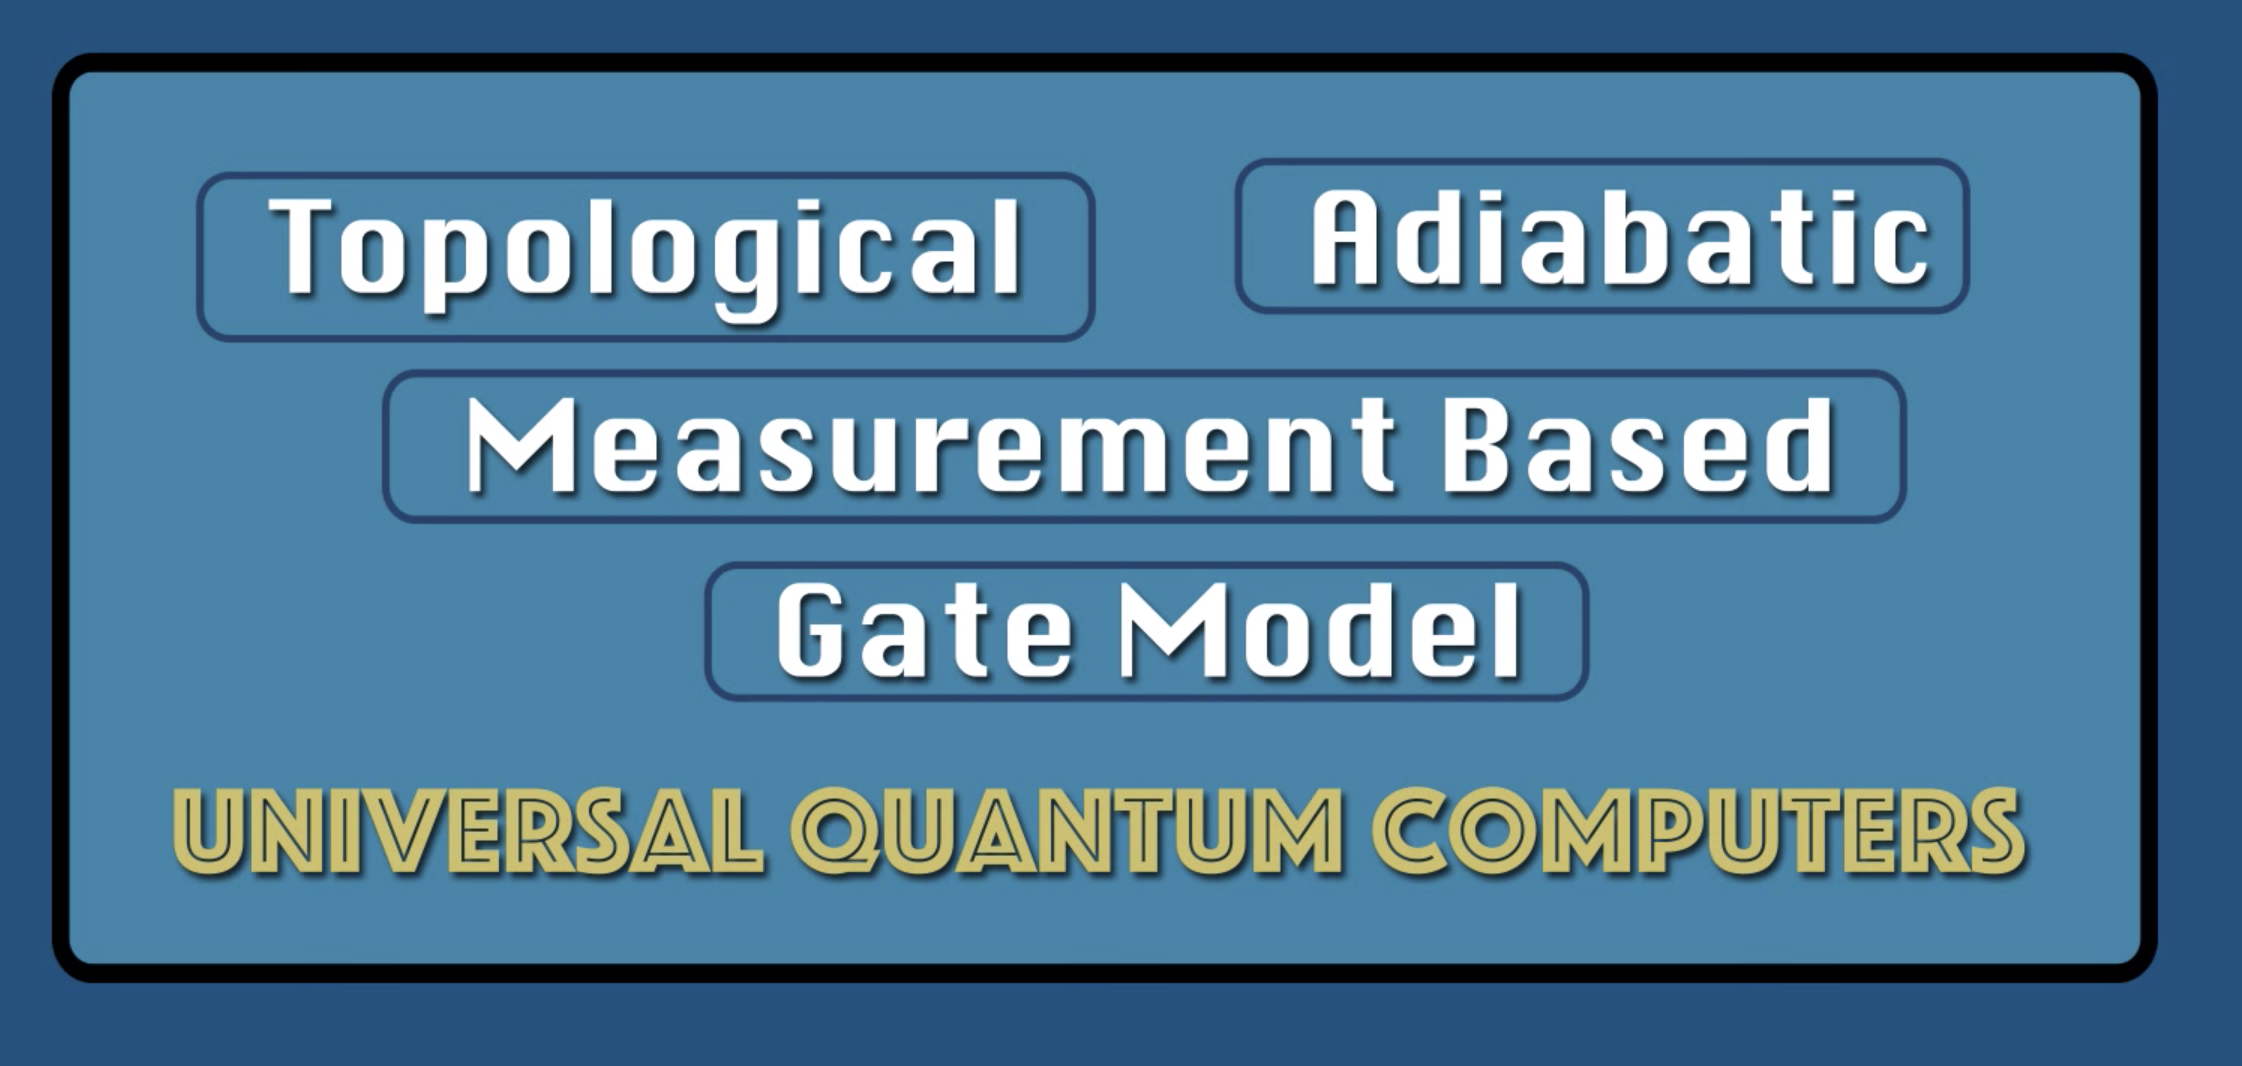
\includegraphics[width=8cm]{uqc.png}
  \caption{Universal Quantum Computers}
  \label{fig:UniversalQC}
\end{figure}

The first quantum computer was built using gate model approach where we control and manipulate state of the Quantumn bits or qbits to do operations and run algorithms. The Universal Quantum Computer is a one where we gate model approach is able to map to other forms of quantum computing in polynomial time and polynomial resources. Various approaches of qantum computing are:
\begin{itemize}
  \item Circuit Based Quantum Computing
  \item Adiabatic Quantum Commputing
  \item Topological Quantum Computing
  \item Measurement Based Quantum Computing
\end{itemize}

\floatstyle{plain}
\restylefloat{figure}
\begin{figure}[h]
  \centering
  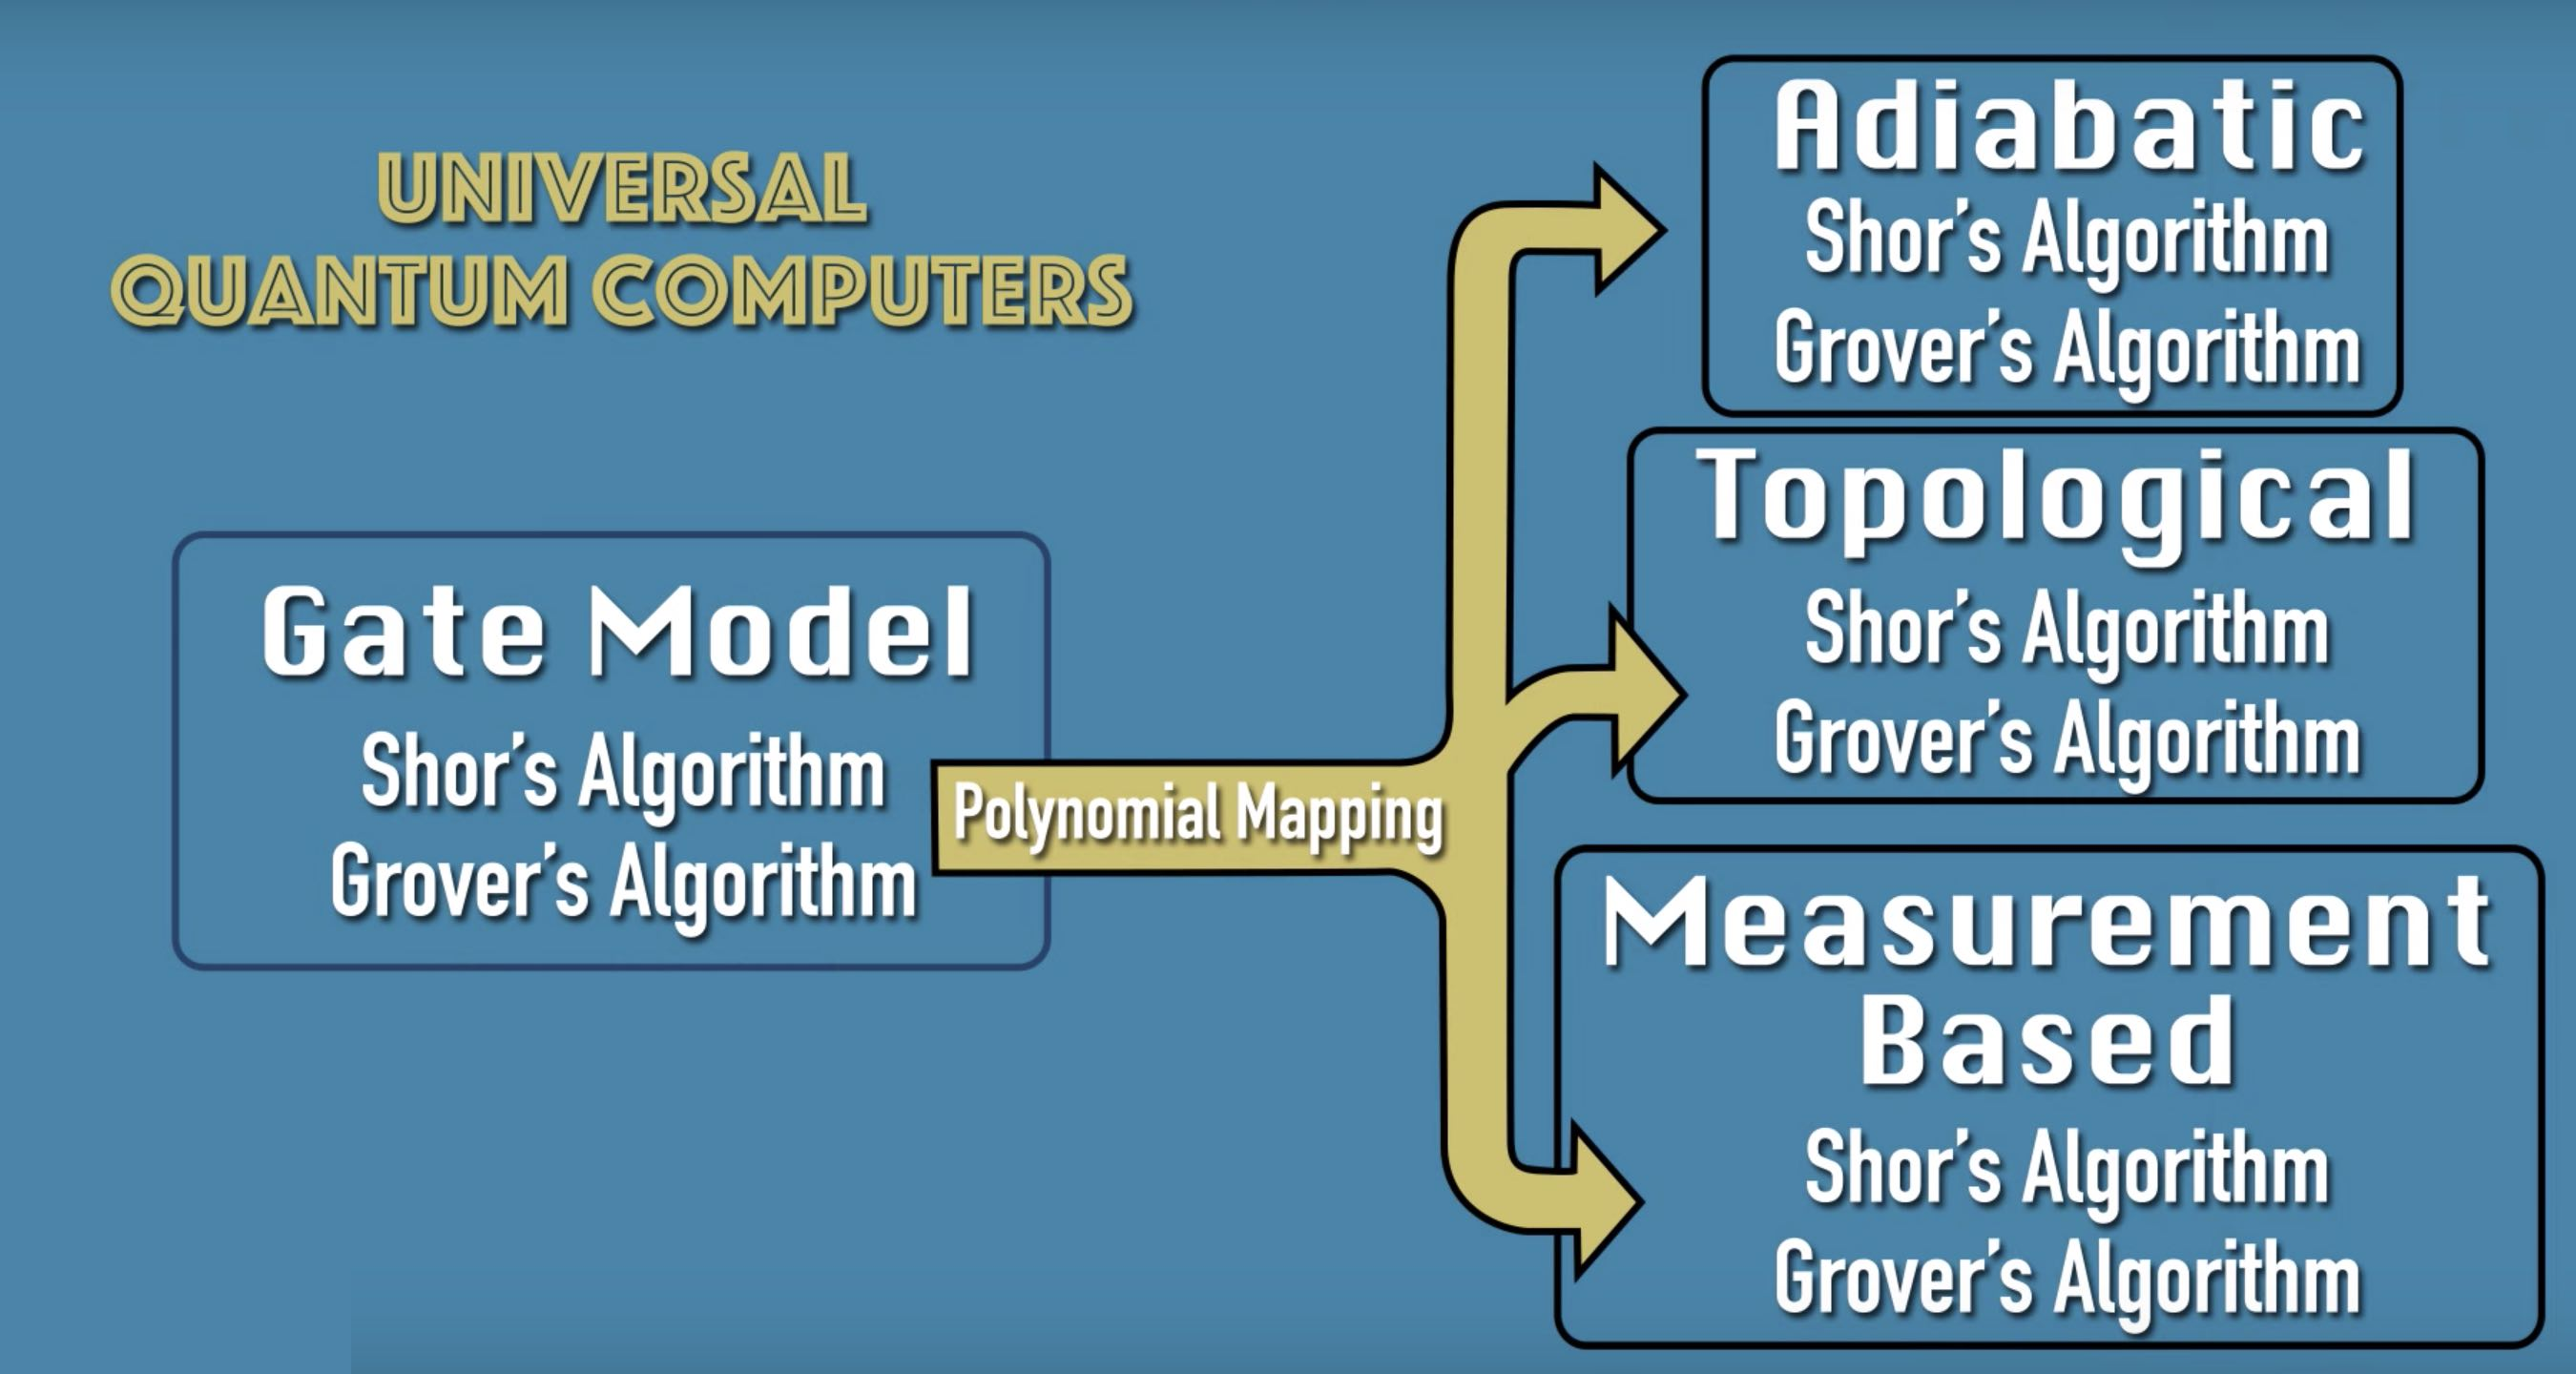
\includegraphics[width=8cm]{uqc_mapping.jpg}
  \caption{Polynomial mapping}
  \label{fig:PolynomicalUQC}
\end{figure}

To be a universal quantum computer, a quantum computer must be able to operate all the above approaches of quantum computing.







\subsubsection{Gates based}
In gate based quantum computing, the gates are built on the principle of qubits: \emph{superposition} and \emph{entanglement}.

\paragraph{Superposition}
Qubit can exist in both 0 and 1 state. It can be represented by the equation:
\begin{equation*}
  \ket {\psi} = a_0 \ket{0} + a_1 \ket{1}
\end{equation*} 
where a\textsubscript{0} and a\textsubscript{1} are configuration that specifies all the possibilities of state being in 0 and 1.

\paragraph{Entanglement}
In quantum computing, in a multi-particle system, entanglement is property of qubits where the state of one qubit cannot be described independently. To express the state of system with two Particles A and B, the quantum state can be described as tensor product of two state space described by the equation:
$\ket {\Phi} = \ket{A} \otimes \ket{B}$
or, it can be also written as
$\ket {\Phi} = \ket{AB}$


\subsubsection{Adiabatic Quantum Computer}
Adiabatic quantum computing is based on Hamiltonian framework for quantum mechanics. Quantum systems evolves by unitary operators. We find the initial easily implementable Hamiltonian H\textsubscript{0}, find a path H\textsubscript{t} and find the final Hamiltonian H\textsubscript{1} keeping the system in ground state which depends on eigen gap. The basic principle of the adiabatic quantum computing is: as long as the path is traversed slowly from H\textsubscript{0} to H\textsubscript{1}, the system remains in ground state and the required solution is obtained. If traversed faster, the system jumps state and it results in error. 

\paragraph{Hamiltonian Formula} 
The Hamiltonian formula can be simplified as follows:
\begin{multline*}
  \mathcal{H}_s(s) = \frac{-1}{2} \sum_i \Delta (s) \sigma_i^x  \\ + \epsilon(s) ( - \sum_i h_i \sigma_i^z + \sum_{i<j} J_{ij}  \sigma_i^z \sigma_j^z)
\end{multline*}
which can be broken down as:
\begin{itemize}
  \item[$-$] $\mathcal{H}_s(s)$ is the required Hamiltonian energy.
  \item[$-$] $[\frac{-1}{2} \sum_i \Delta (s) \sigma_i^x]$ is the initial Hamiltonian, where all the qubits are in superposition state.
  \item[$-$] $ \epsilon(s) ( - \sum_i h_i \sigma_i^z + \sum_{i<j} J_{ij}  \sigma_i^z \sigma_j^z)$ is the final Hamiltonian, the answer to the problem, which contains the biases and couplers.
\end{itemize} 
One thing to note is that the initial states are Quantum states and the final states are classiscal states.

\paragraph{Eigen Value and Anti-crossing}
In adiabatic system, the systems stays in ground state through out the cycle of getting solution. Staying in ground state depends on speed of traverseing, if too fast or the thermal energy from physical systems. The system initially is at 0 enery level and at the end, it is at zero energy level. During the process, the systems's state might jump and escape from ground state to higher energy state based on the energy gap between two states, which is called anti-crossing and Eigen value of states.

\section{Quantum Annealing for problems}
Quantum Annealing is done using the adiabatic quantum computing approach.

A qubit can exist in two state due to superposition initially, 0 or $\downarrow$  spin and 1 or $\uparrow$. The energy state at superposition is lowest. 
\floatstyle{plain}
\restylefloat{figure}
\begin{figure}[h]
  \centering
  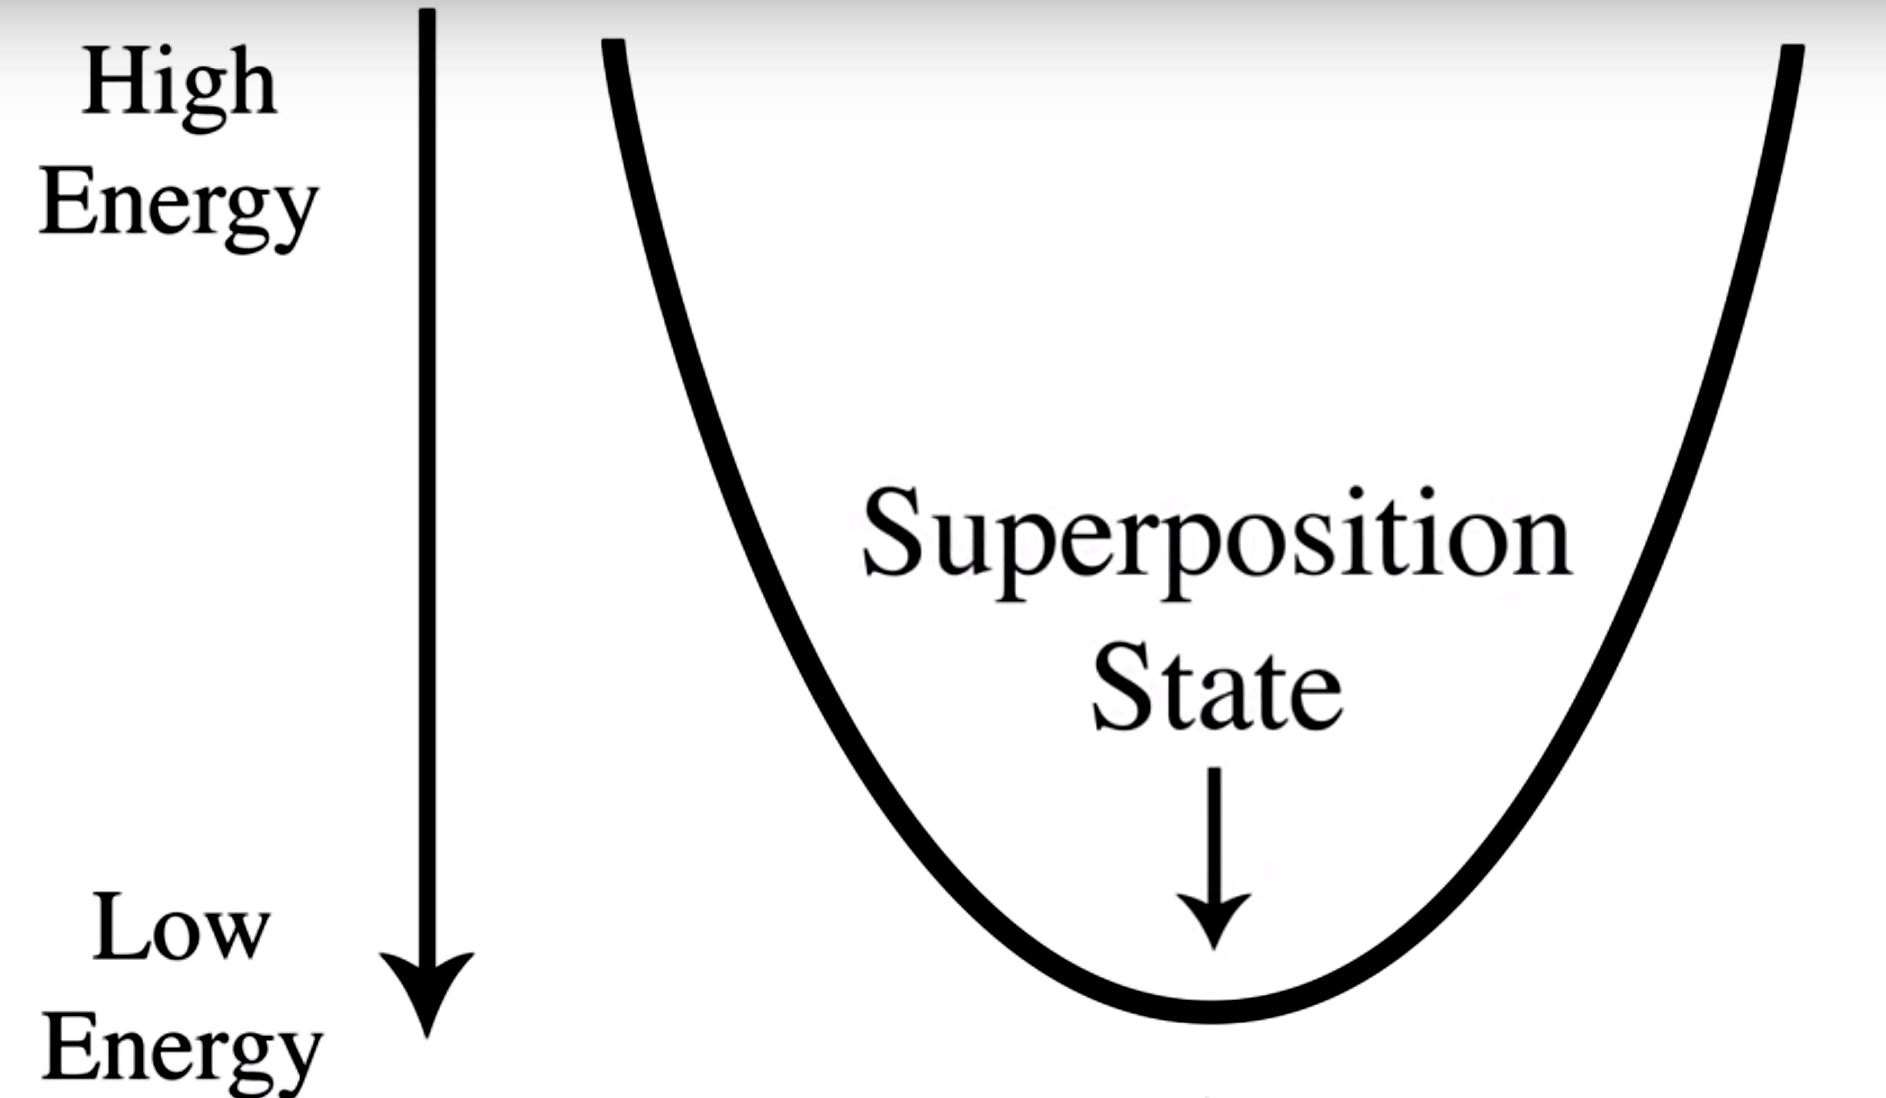
\includegraphics[width=5cm]{sp-energy.png}
  \caption{Superposition qubit energy}
  \label{fig:SPQbitE}
\end{figure}

Once quantum annealing is applied, each qubit goes into either 0 or 1 state, ie classical state, the energy is represented by a double well potential diagram.
 
\floatstyle{plain}
\restylefloat{figure}
\begin{figure}[h]
  \centering
  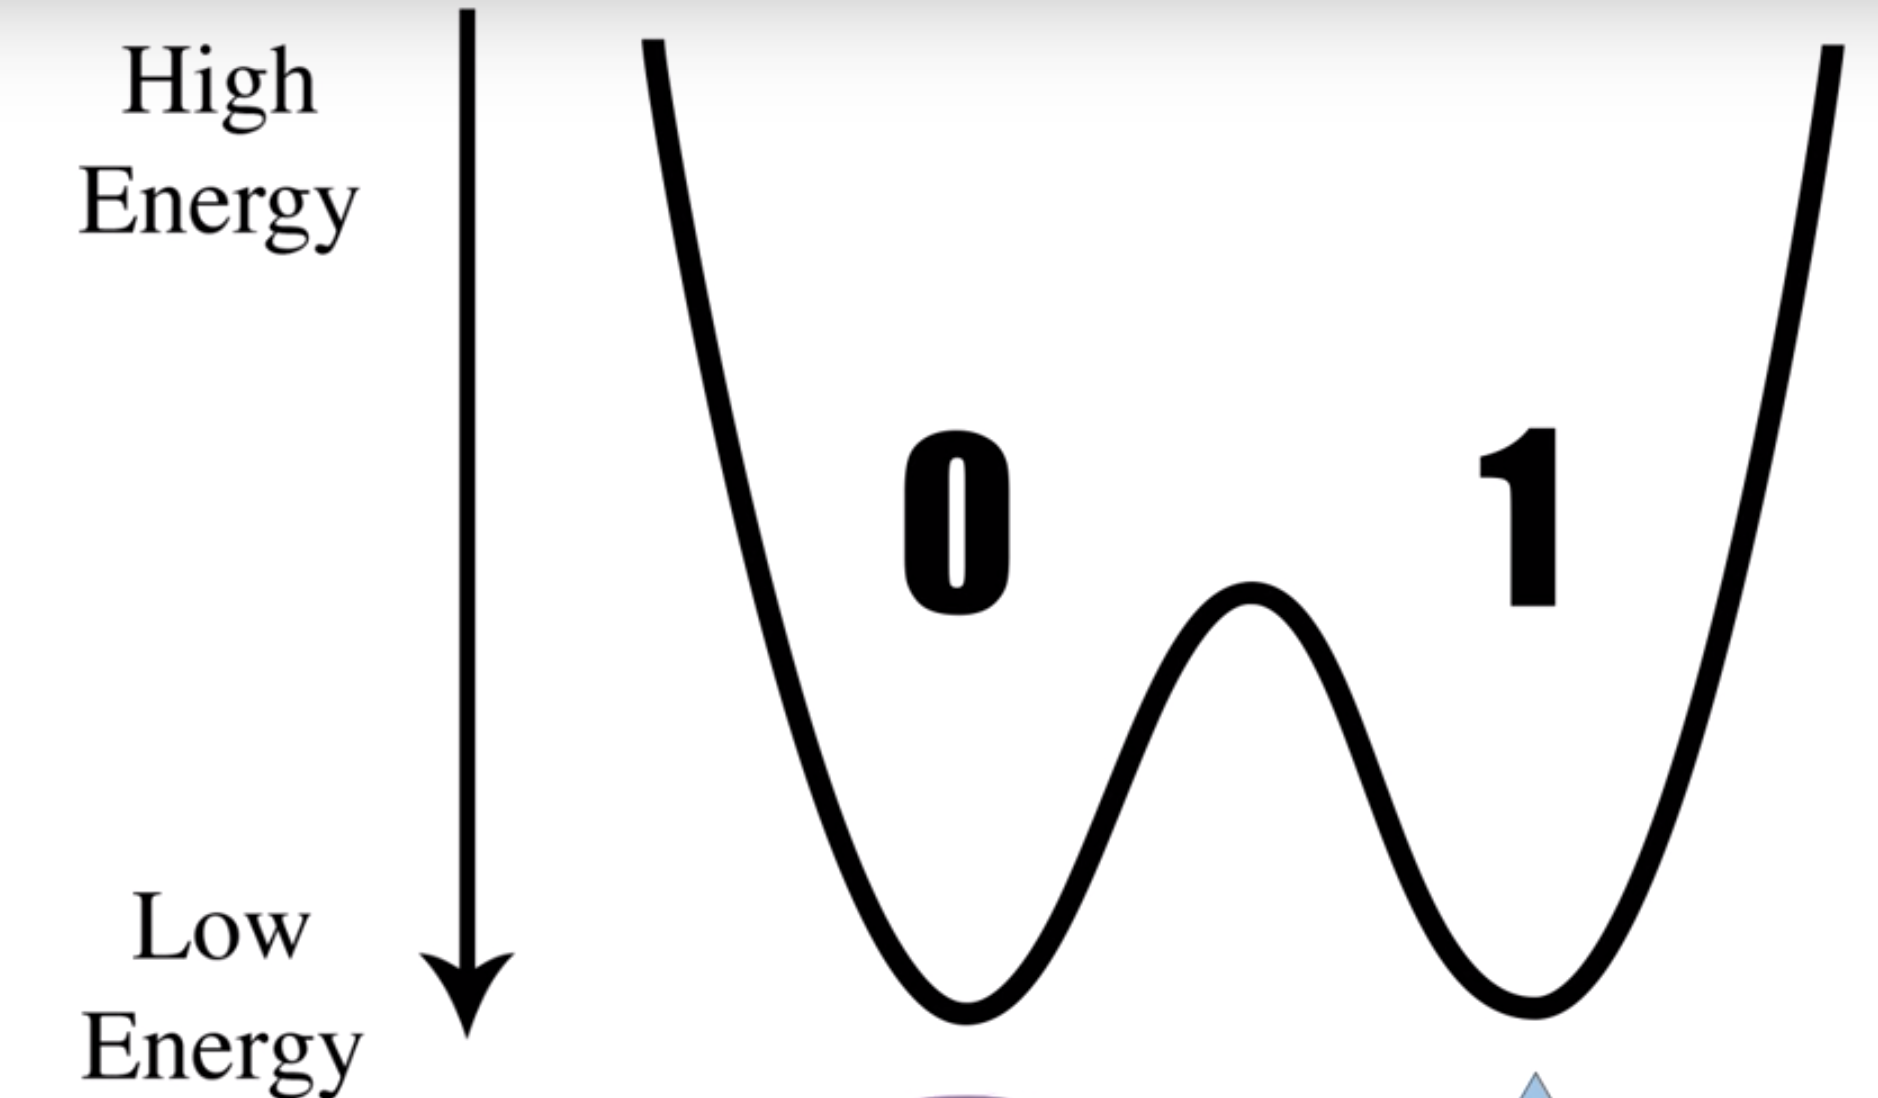
\includegraphics[width=5cm]{qubit_energy.png}
  \caption{Double well potential of a qubit}
  \label{fig:DQPQbit}
\end{figure}

To get the desired answer, the energy of this double well potential is controlled by influence of a magnetic field, known as \emph{bias}. 
 
\floatstyle{plain}
\restylefloat{figure}
\begin{figure}[h]
  \centering
  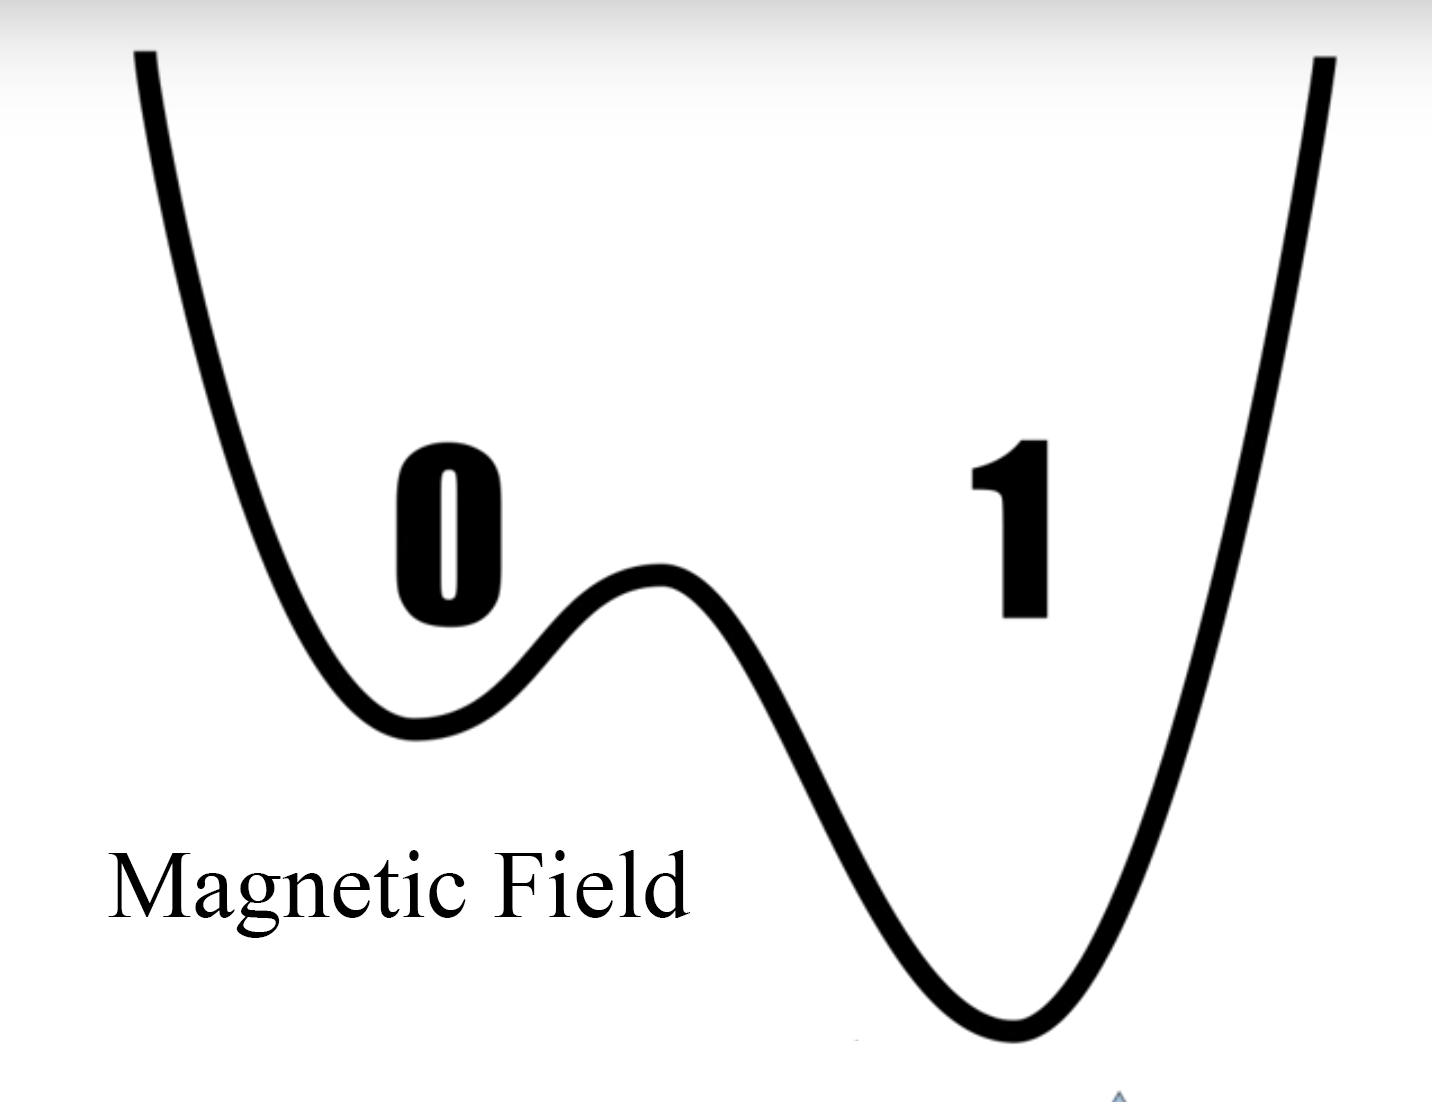
\includegraphics[width=5cm]{qubit_mag.png}
  \caption{Biased qubit double well potential}
  \label{fig:BDQPQbit}
\end{figure}
 
To influence all the qubits in system, qubits are linked by the entanglement property of qubits. This linking is called \emph{coupling}. There are two types of coupling: 0-0 or 1-1 coupling and 1-0 or 0-1 coupling. 

\floatstyle{plain}
\restylefloat{figure}
\begin{figure}[h]
  \centering
  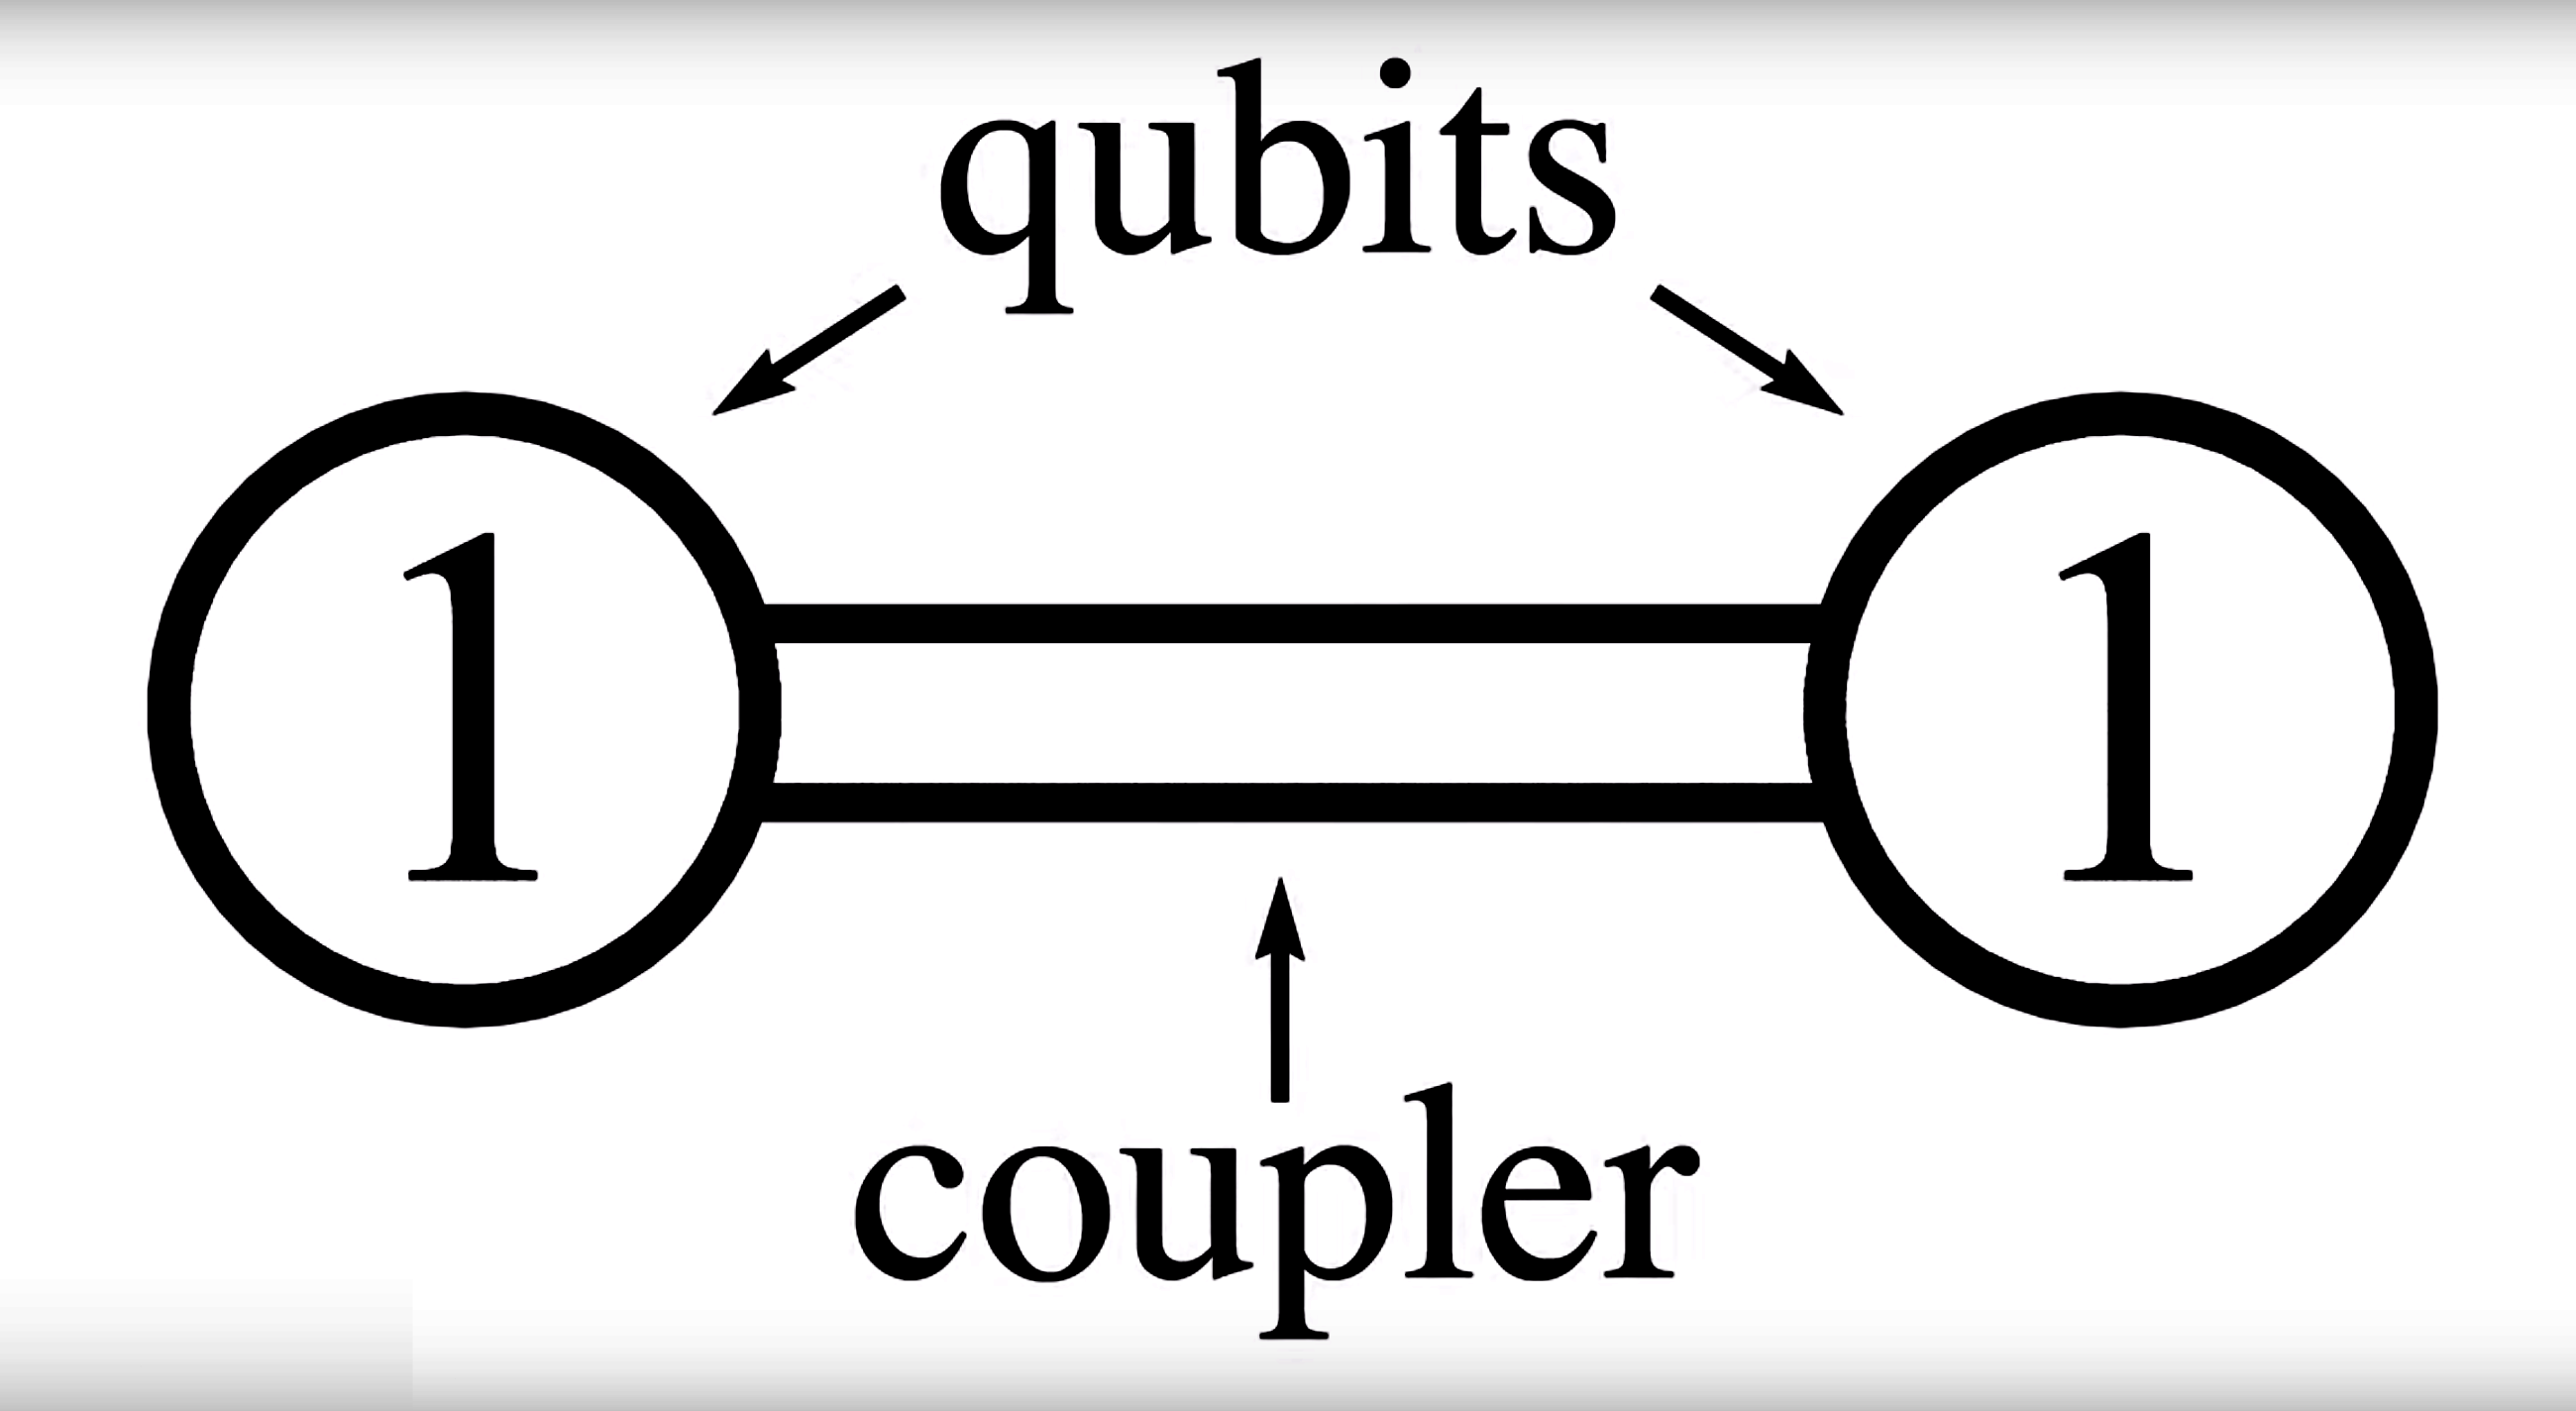
\includegraphics[width=5cm]{qubit_couplet.png}
  \caption{Coupling between two qubit}
  \label{fig:QbitC}
\end{figure}

Hence the potential of this coupled qubits depends on biases of each qubits and the coupling between them. They can be present in either 00,01,10 or 11. The outcome is controlled by the problem we define, at the end the answer is the lowest potential state of the two qubits. Taking all the qubits into account, we get a energy landscape, where the minima on energy cure is the answer ti the problem we are solving. 

\floatstyle{plain}
\restylefloat{figure}
\begin{figure}[h]
  \centering
  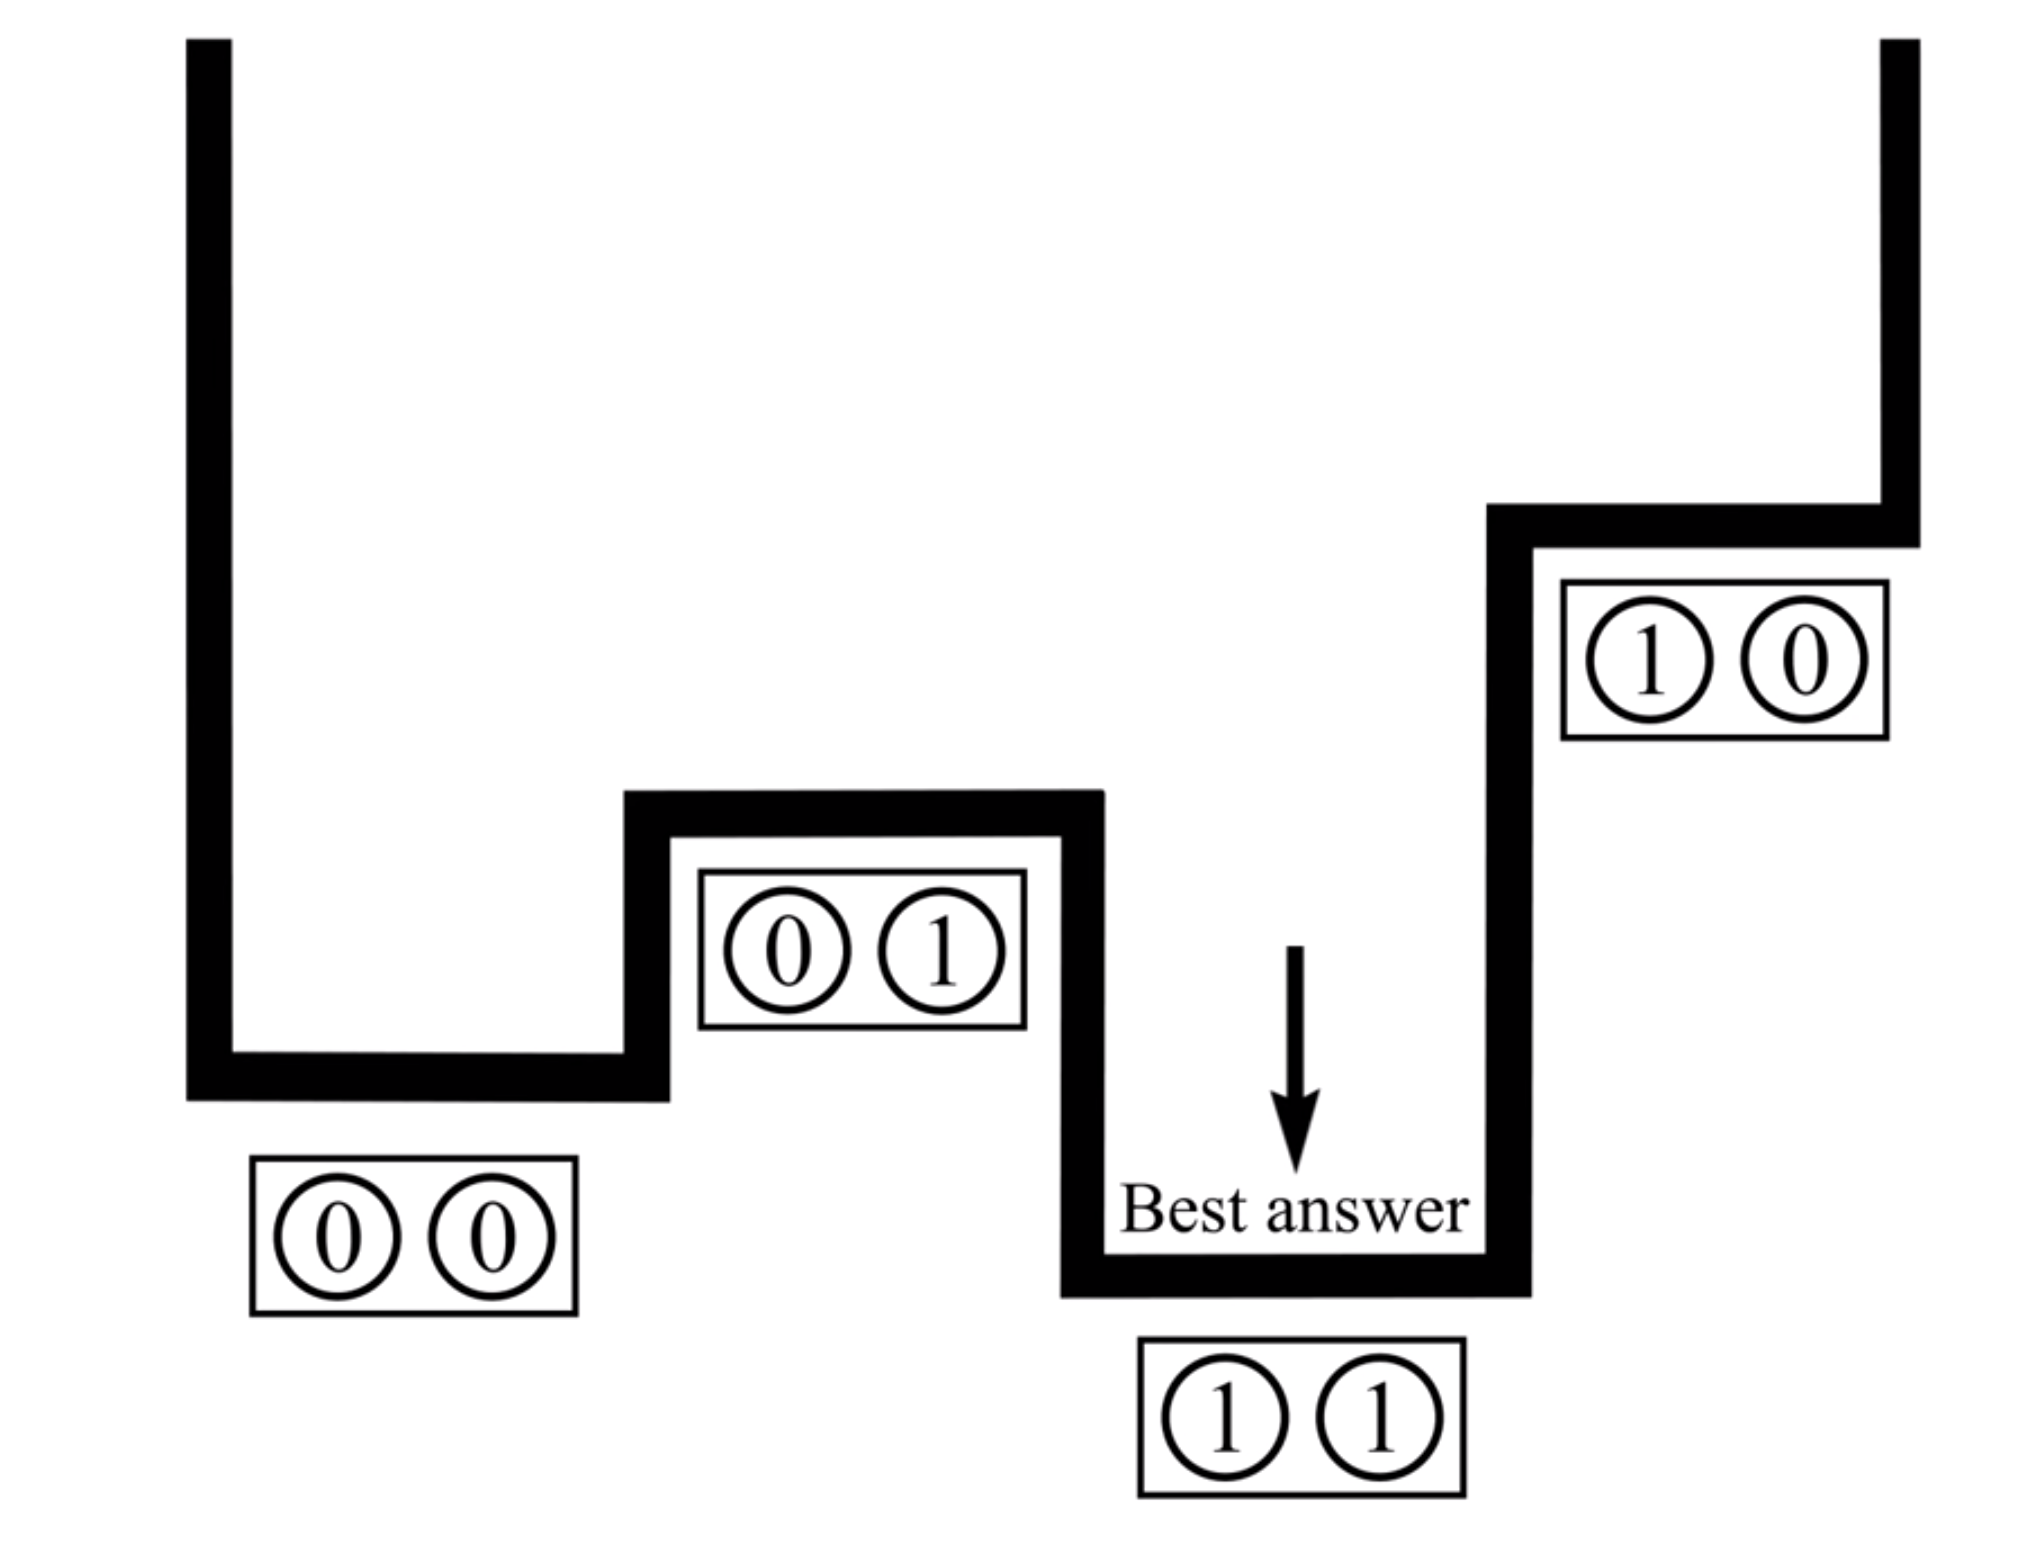
\includegraphics[width=5cm]{entangled_low.png}
  \caption{Double well potential of a qubit}
  \label{fig:ELQbit}
\end{figure}

The combination (C) of states of a quantum computer for quantum annelaing depends on number of qubits (n) defined as: $ C = 2^n$.

To compare this with universal gate based quantum computer, the main difference lies in the way a problem is solved. In gate based quantum computer, the states of individual qubits is controlled and the solution is obtained. In quantum annealing, the problem is formulated, desired Hamiltonian is calculated, finally the system after going through annealing schedule\cite{1}, calculates the solution, which is the minima on energy curve of the ground state of quantum system. Quantum annealing is useful for optimization problem, where the goal is to get best possible solution with lowest cost. Quantum annealing is not good to solve search algorithms like Grover's search algorithm. 

\section{D-Wave systems and using its SDK and Cloud}
D-Wave Systems Inc has been developing quantum computers, which currently offers quantum computer with 2038 Qubits, which works on the principle of quantum annealing, as explained above. Quantum annealing can be used for areas including:
\begin{itemize}
  \item[$-$] Optimization 
  \item[$-$] Machine learning
  \item[$-$] Cybersecurity
  \item[$-$] Image analysis
  \item[$-$] Pattern recognition
  \item[$-$] Financial rnalysis
  \item[$-$] Bioinformatics/cancer research
  \item[$-$] Trafic flow 
  \item[$-$] Manufacturing Process
\end{itemize}

The system is based on superconducting device at absolute zero temperature.

\paragraph{Ocean SDK} D-Wave offers Ocean SDK which has a set of tools to run,simulate and implement quantum algorithms. The D-Wave system provides a quantum processing unit (QPU) to solve a binary quadratic model (BQM). The are advanced features and tools for further improvements of the solution. There are numerous tools provided in the SDK including binary and quadratic sampler, annealing sampler, Ising problems micro-embedding. Some of the examples are available online on github and on ocean's doc website. 

\paragraph{LEAP} Leap is a real time environment from D-Wave which provides tools and access to quantum computing in cloud to its uses. It has interactive examples which explains implementation of integer factoring problem and structural imbalance problem with cases, and comparision of time taken to solve it on D-Wave vs classical computer.

\floatstyle{plain}
\restylefloat{figure}
\begin{figure}[h]
  \centering
  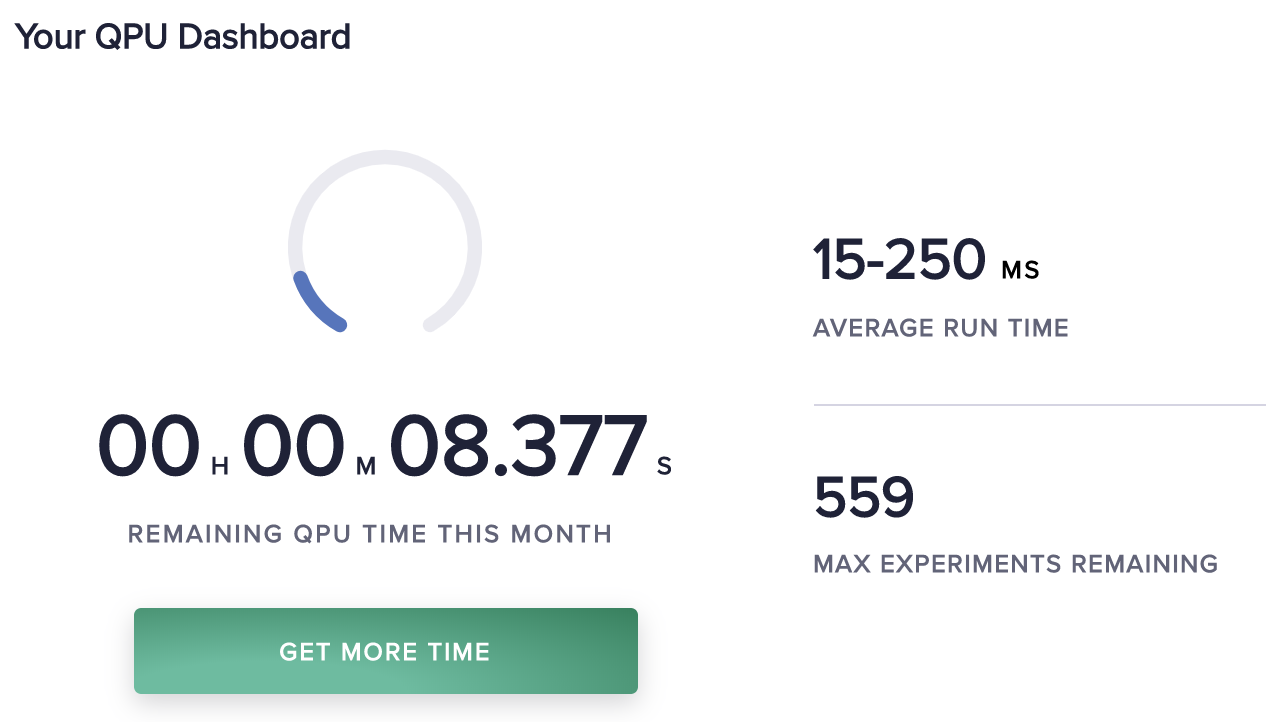
\includegraphics[width=8cm]{Leap-db1.png}
  \caption{Leap Dashboard 1}
  \label{fig:LDB}
\end{figure}

\floatstyle{plain}
\restylefloat{figure}
\begin{figure}[H]
  \centering
  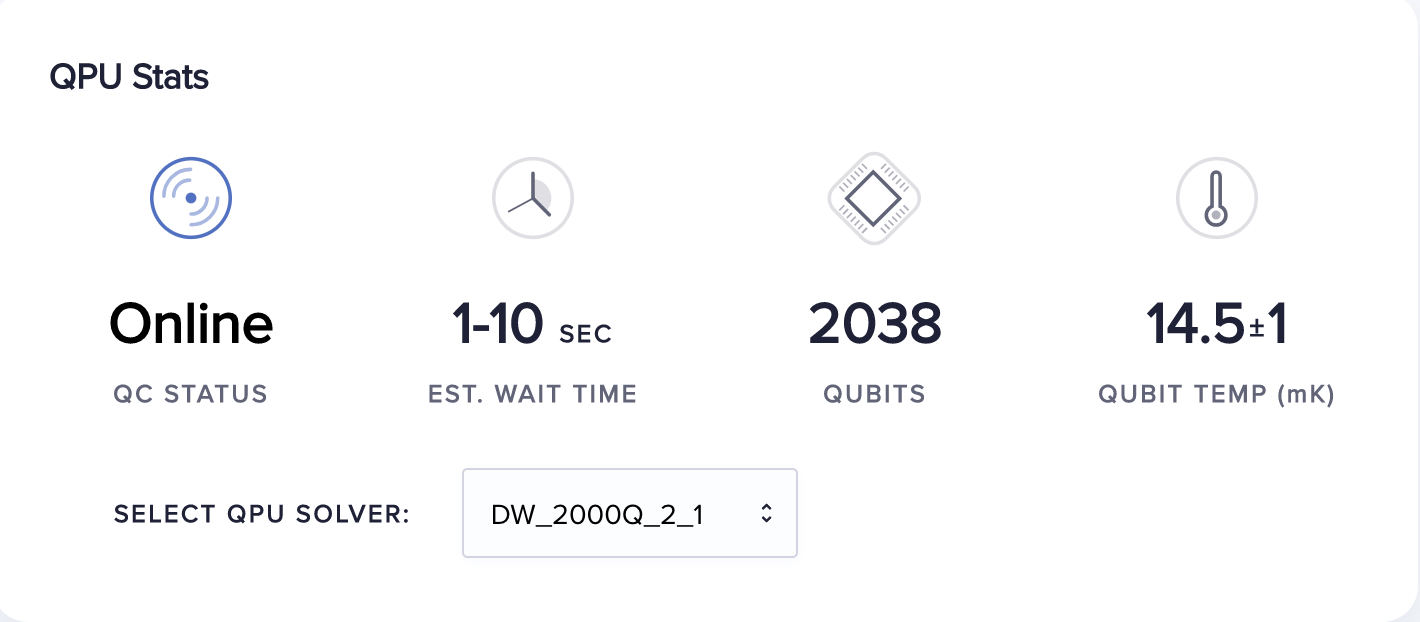
\includegraphics[width=8cm]{Leap-db2.png}
  \caption{Leap Dashboard}
  \label{fig:LDB2}
\end{figure}



\section{Experimentation}
To experiment with D-Wave system, we tried to use the LEAP system and run Integer Factoring and Structural Imbalance problem. Besides LEAP, we implemented demo examples from Ocean SDK, both of which can be found on the github and in documents.


\subsection{Map Coloring}
This example is implemented using D-Wave's Ocean SDK. 

Map coloring problem is a constraint satisfaction problem. The primary requirement of a constraint satisfaction problem is to find a result from finite set of domain, values are assigned to a problem, staisfying all constraint. 

In map coloring example, all regions are to be colored and the constraint is that for any neighbouring regions, the color should not be same. In this case, the regions are states of Canada.

To implement this using Ocean SDK, we followed and used the example given on D-Wave's documentation. The steps briefly to solve the problem are: 

\begin{itemize}
  \item Formulate problem as graphic
  \item Create binary constraint satisfaction problem
  \item Convert to binary quadratic model (BQM)
  \item Sample using D-Wave SAPI solver
  \item Plot a valid solution.
\end{itemize}

\subsection{Integer Factoring}
\hfill $\sum_i^N q_ix_i + \sum_{i<j}^N q_{i,j}x_i  x_j$
Subsubsection text here.

\subsection{Structural Imbalance}
Subsubsection text here.

\section{Experience and Result}
Quantum annealing proves to be useful in general to solve problems and find solution in terms of time required as compared to a quantum computer. D-Wave's Ocean SDK and LEAP is useful tool to learn quantum annealing and how to practically use it and implement to solve problems. It provides an insight to how just using adiabatic quantum computing approach, number of qubits can be increased in a quantum computer as compared to a universal gate based quantum computer and the advantages and disadvantages of adiabatic quantum computing. 

Setting up Ocean SDK gives the connection to D-Wave's QPU (Quantum Processing Unit).

\floatstyle{plain}
\restylefloat{figure}
\begin{figure}[h]
  \centering
  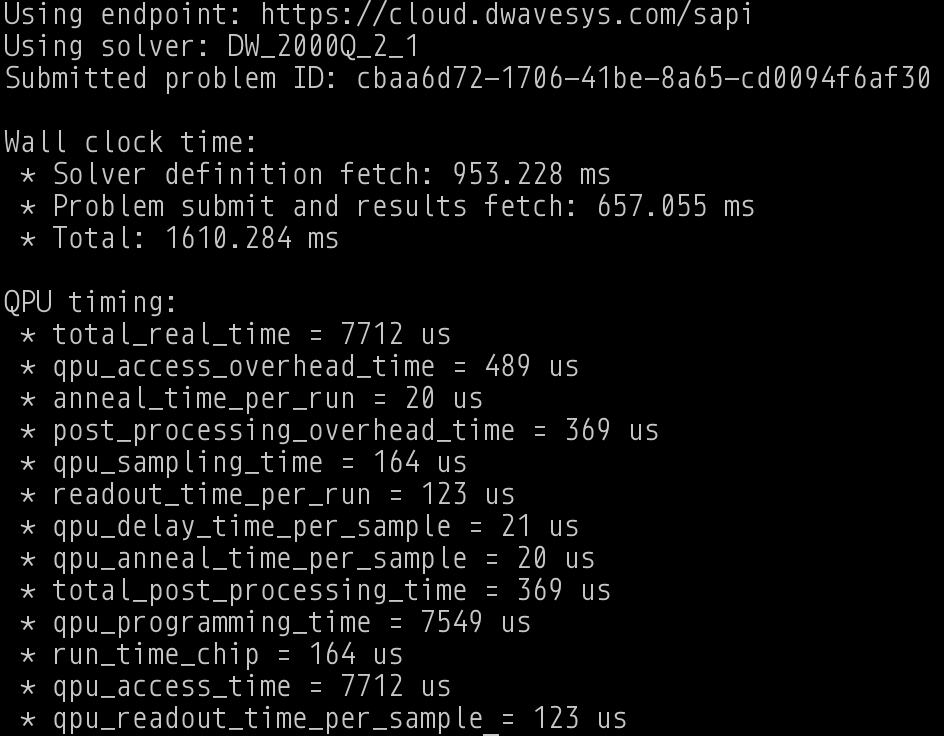
\includegraphics[width=8cm]{sdk.png}
  \caption{Ocean SDK ping status}
  \label{fig:OSDK}
\end{figure}


The result for the algorithms implemented above are shown below. 

\subsection{Map Coloring Problem}

For map coloring problem, the following graph plot was obtained.
\floatstyle{plain}
\restylefloat{figure}
\begin{figure}[h]
  \centering
  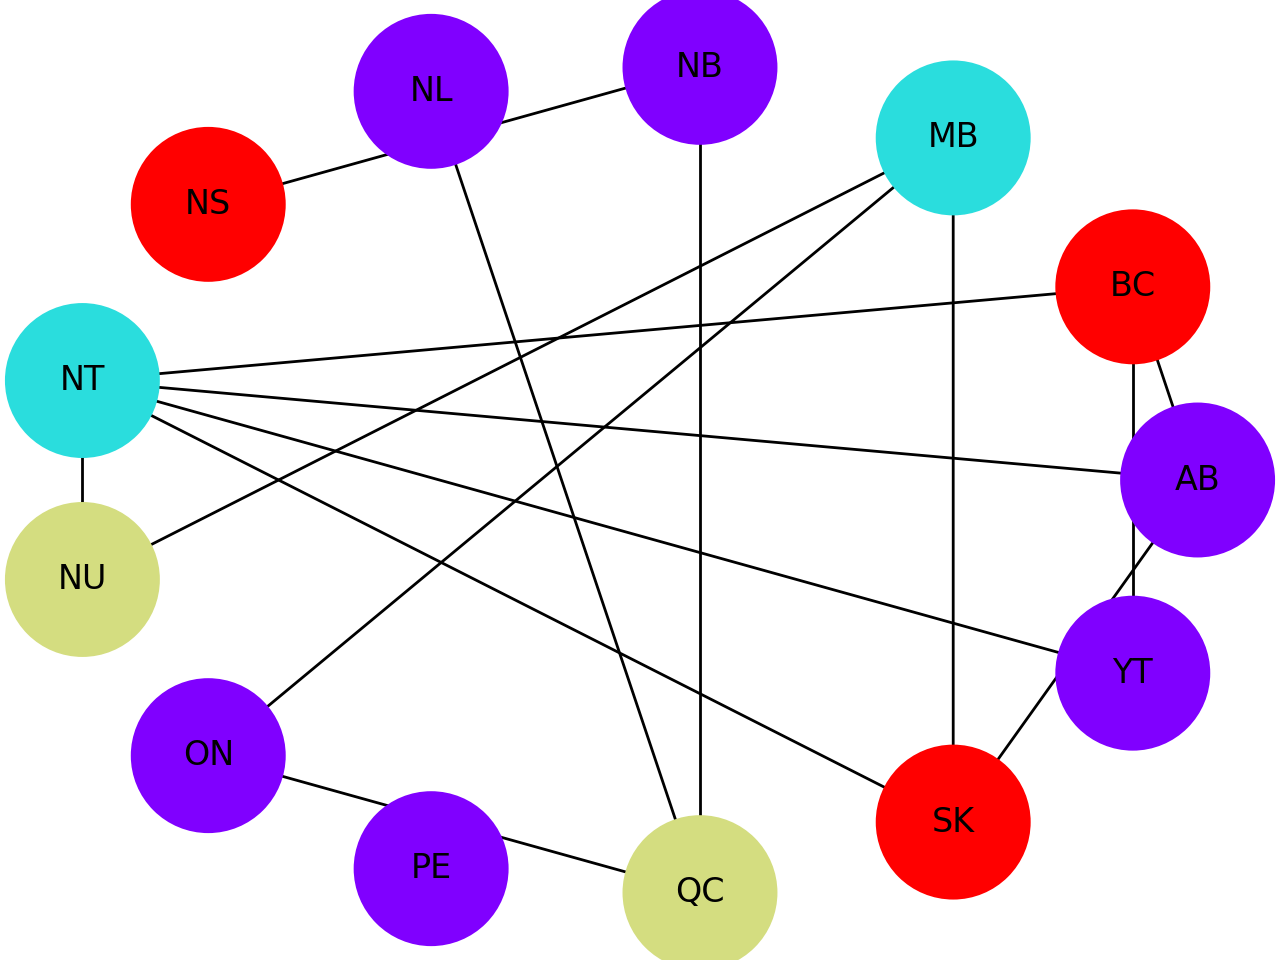
\includegraphics[width=6cm]{map_coloring.png}
  \caption{Map Coloring Solution}
  \label{fig:MCS}
\end{figure}


\section{Future Steps}
All the work that was carried out is in regards to Quantum Annealing. For next steps we want to try out all the available advanced features on D-Wave and implement advanced algorithms to solve problems. 

\section{Conclusion}
D-Wave's quantum computer are powerful quatum computer for quantum annealing. The resoures and example given can be easily understood and implemented. Quantum Annealing is useful to solve problem where the best possible solution is required. This feature can also be used in machine learning, authentication and validation and analysis. Using leap's interactive examples, we understand how solving these problems compare on a classical computer versus a quantum computer and the advantage it provides in terms of time. 

\begin{thebibliography}{1}

\bibitem{IEEEhowto:kopka}
H.~Kopka and P.~W. Daly, \emph{A Guide to}, 3rd~ed.\hskip 1em plus
  0.5em minus 0.4em\relax Harlow, England: Addison-Wesley, 1999.

\end{thebibliography}

\appendix

\subsection{First Appendix}
\label{FirstAppendix}

\subsubsection{First Subsection In Appendix}
\label{FirstSubsectionAppendix}

\subsection{FIGURES AND TABLES}

\listoffigures

% that's all folks
\end{document}


